\subsection{Caméra embarquée}
\label{subsec:camera_elec}

Le système de caméras embarquées a pour objectif de documenter le déroulement du vol et les principaux événements de la
mission. Chaque étage emporte deux caméras. Le premier étage comporte une caméra orientée vers l'horizon et une caméra située
à l'intérieur de la séparation inter-étages. Le deuxième étage comporte deux caméras orientées en mode portrait : l'une filme
l'horizon et l'autre le sol.

\subsubsection{Caméras retenues}

Le choix des caméras a évolué au cours du développement. La caméra initialement prévue pour observer la séparation depuis le
premier étage était une Arducam de résolution de 2 mégapixels, équipée d'un capteur \verb|OV2640|. Cette solution devait
permettre à un microcontrôleur de récupérer le flux vidéo et de l'enregistrer sur une carte SD. Elle a cependant été abandonnée
avant le vol au profit d'une RunCam Nano 2. Cette dernière est plus compacte, plus simple à mettre en œuvre et plus fiable dans
le contexte du projet. Elle ne nécessite notamment pas de développer une chaîne logicielle dédiée à la récupération et à
l'enregistrement de la vidéo.

\begin{figure}[H]
    \centering
    \begin{subfigure}{0.3\textwidth}
        \centering
        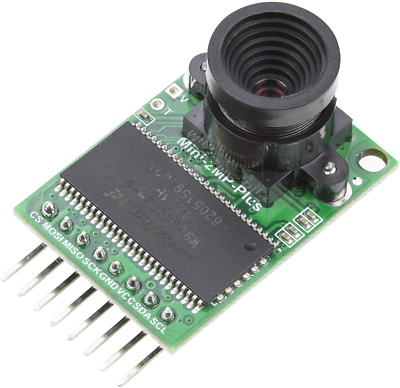
\includegraphics[width=0.95\linewidth,height=3.2cm,keepaspectratio]{figures/s-l400.png}
        \caption{Arducam OV2640}
        \label{subfig:camera_arducam}
    \end{subfigure}
    \hfill
    \begin{subfigure}{0.3\textwidth}
        \centering
        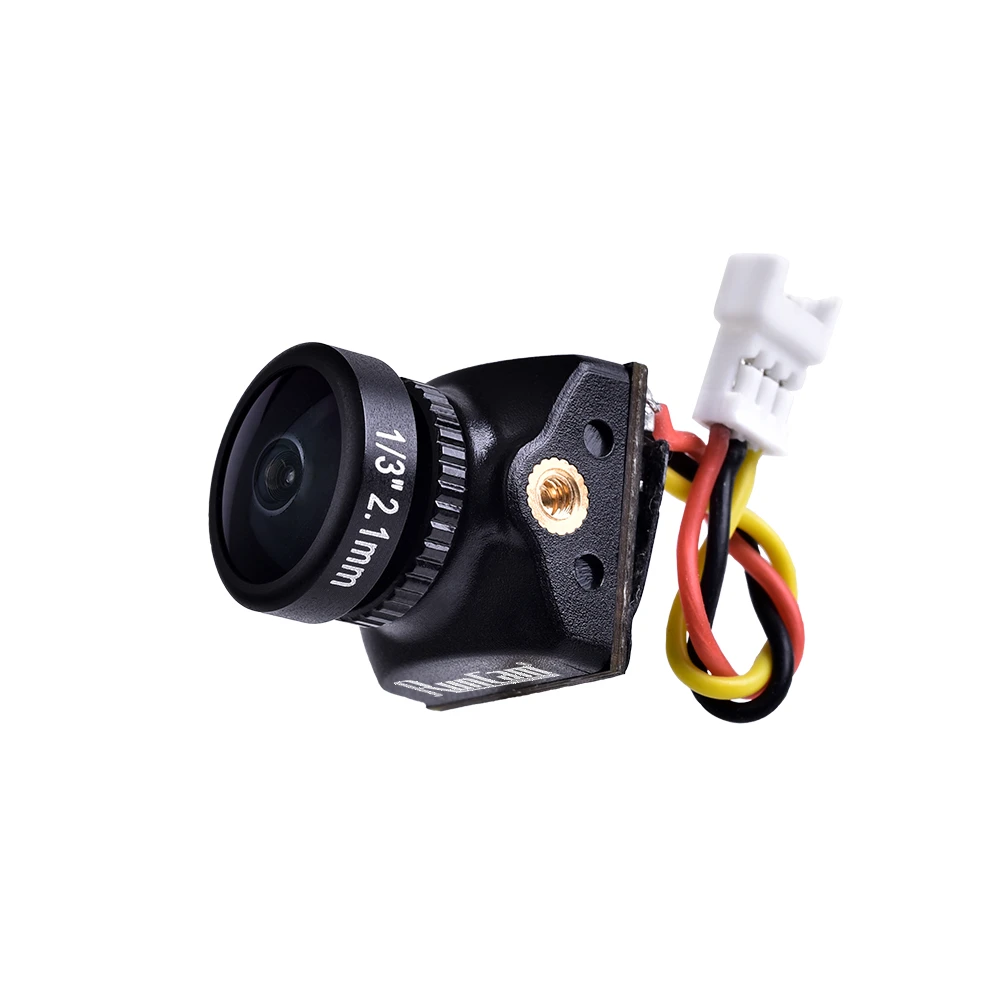
\includegraphics[width=0.95\linewidth,height=3.2cm,keepaspectratio]{figures/nano2.png}
        \caption{RunCam Nano 2}
        \label{subfig:camera_nano2}
    \end{subfigure}
    \hfill
    \begin{subfigure}{0.3\textwidth}
        \centering
        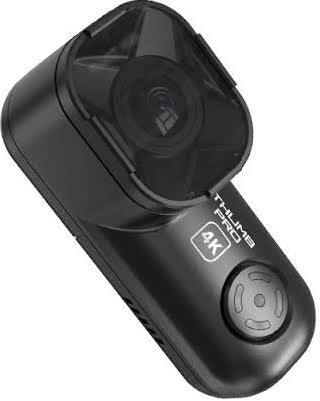
\includegraphics[width=0.95\linewidth,height=3.2cm,keepaspectratio]{figures/thumb.jpeg}
        \caption{RunCam Thumb Pro}
        \label{subfig:camera_thumb}
    \end{subfigure}
    \caption{Caméras étudiées et utilisées pour le système embarqué.}
    \label{fig:camera_models}
\end{figure}

\begin{figure}[H]
    \centering
    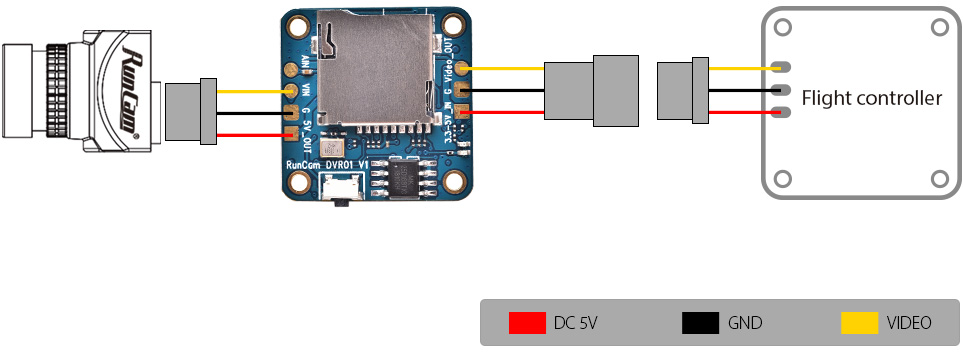
\includegraphics[width=0.85\textwidth]{figures/RC-DVR-2.jpg}
    \caption{Architecture du système associant la RunCam Nano 2, son DVR et la PCB dédiée aux caméras.}
    \label{fig:camera_nano2_dvr}
\end{figure}

Dans cette architecture, le terme \og flight controller \fg{} désigne la PCB dédiée aux caméras. Le flux vidéo ne transite pas
par cette carte : la RunCam Nano 2 transmet directement le signal vidéo analogique au DVR, qui assure seul son acquisition et
son enregistrement. La PCB caméra ne fournit donc que l'alimentation et le signal de commande de la caméra.\\

Un risque de perturbations électromagnétiques a toutefois été identifié lors du choix de cette solution. Lors de précédents
projets, l'utilisation d'une RunCam Nano avait montré que le signal vidéo analogique, transmis en PAL à haute fréquence entre la
caméra et le DVR, pouvait perturber l'électronique située à proximité. Une perturbation du récepteur GNSS avait notamment été
observée. La RunCam Nano 2 et son DVR étant installés dans la séparation inter-étages, cette contrainte a pu être maîtrisée.
Cette séparation est constituée d'une pièce en aluminium et deux plaques d'aluminium de \SI{3}{\milli\meter} séparent le DVR
de l'électronique de la baie avionique. Ces éléments assurent un blindage suffisant pour écarter le risque de perturbation de
l'électronique environnante. La Nano 2 a ainsi pu être retenue malgré la nature analogique de sa liaison vidéo, l'architecture
mécanique de la fusée fournissant la protection nécessaire.

\subsubsection{Carte de commande et interfaces}

Une carte électronique dédiée au système de caméras a été conçue et assemblée. Elle est équipée d'un ESP32 Xiao C3, qui assure la
gestion des commandes des caméras. La conception initiale était prévue pour l'Arducam : le microcontrôleur devait récupérer les
données vidéo par une interface SPI/I2C et les enregistrer sur une carte SD partageant le bus SPI. La complexité de cette
architecture, ainsi que la charge de calcul et la quantité de code nécessaires, ont conduit à modifier la solution après
l'assemblage des cartes.\\

Les deux caméras de chaque étage sont reliées à leur PCB caméra respectif. Pour intégrer la RunCam Nano 2 sans reconcevoir la
carte, les connexions déjà prévues pour l'Arducam ont été réutilisées. La ligne initialement destinée au signal CS du bus SPI a
été affectée au signal de commande High/Low de la Nano 2. Les lignes d'alimentation 5 V et GND ont également été conservées
pour alimenter cette caméra. Le DVR de la Nano 2 étant autonome, aucune acquisition ni aucun stockage vidéo supplémentaire
n'est réalisé par la carte. Les RunCam Thumb Pro et la RunCam Nano 2 enregistrent directement les vidéos sur leurs cartes SD.
La capacité disponible est supérieure à la durée d'autonomie des batteries. Les caméras créent des fichiers vidéo de
\SI{10}{\minute}, et les fichiers déjà enregistrés sont conservés après la coupure de leur alimentation.

\begin{figure}[H]
    \centering
    \begin{subfigure}[t]{0.48\textwidth}
        \centering
        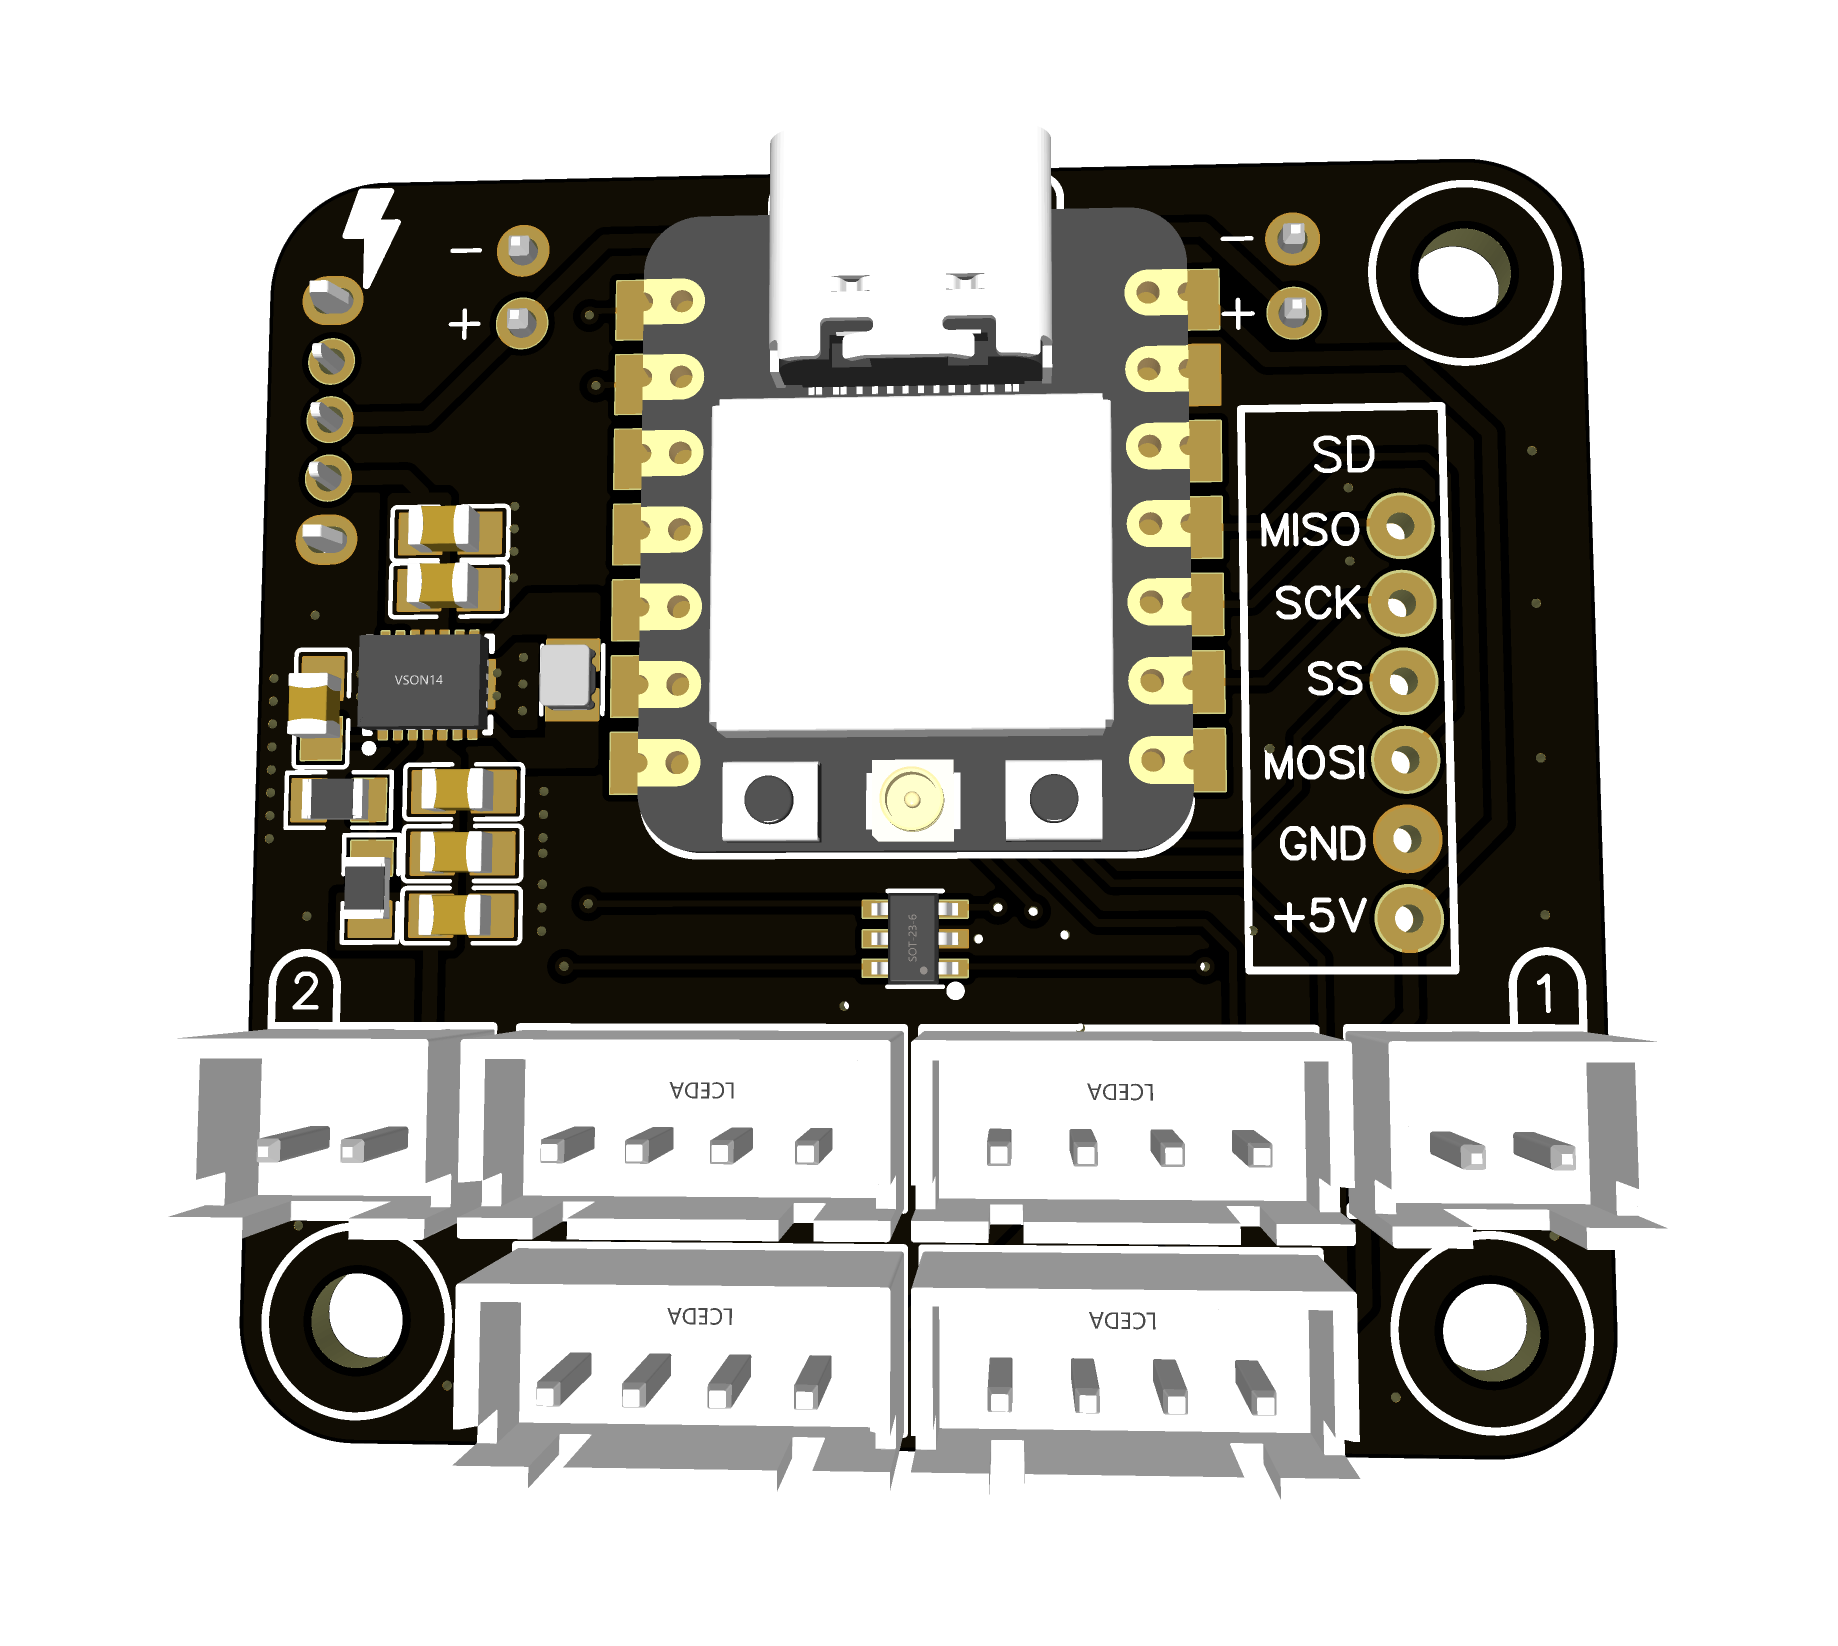
\includegraphics[width=\linewidth]{figures/elec/PCB_camera_A.png}
        \caption{Face A.}
        \label{subfig:pcb_camera_a}
    \end{subfigure}
    \hfill
    \begin{subfigure}[t]{0.48\textwidth}
        \centering
        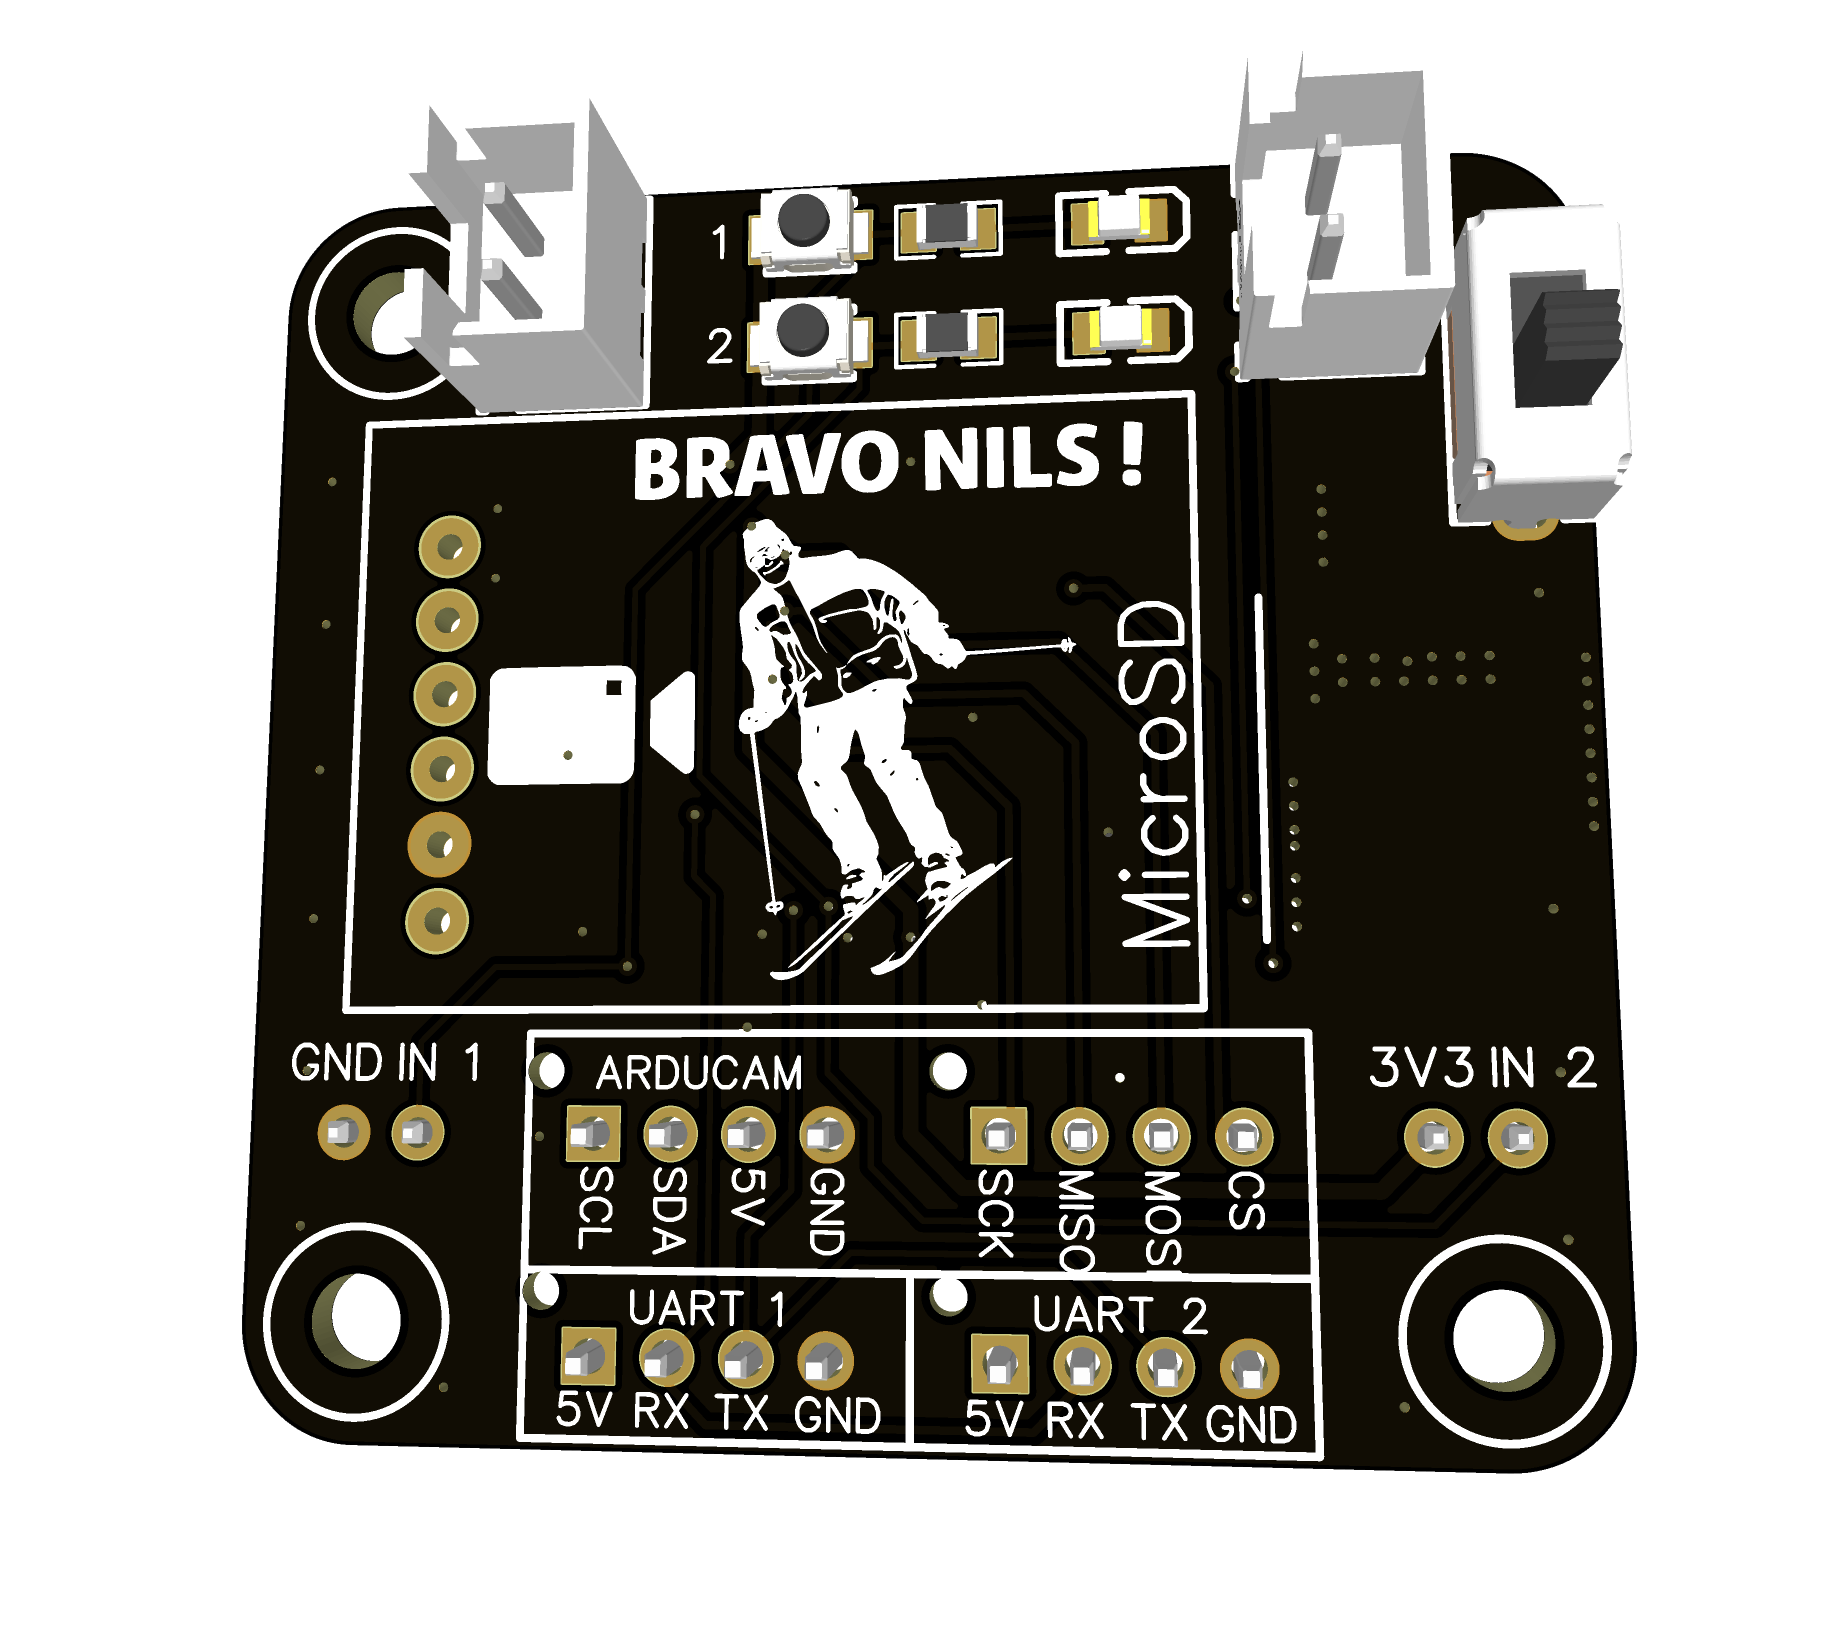
\includegraphics[width=\linewidth]{figures/elec/PCB_camera_B.png}
        \caption{Face B.}
        \label{subfig:pcb_camera_b}
    \end{subfigure}
    \caption{Faces A et B de la PCB dédiée aux caméras.}
    \label{fig:pcb_camera}
\end{figure}

La carte possède deux entrées de commande, nommées IN1 et IN2. Chacune est reliée à un trigger de Schmitt, dont la sortie est
connectée à un GPIO de l'ESP32 Xiao C3. Cette mise en forme permet au microcontrôleur de détecter de manière fiable les
changements d'état des signaux de déclenchement.\\

L'entrée IN1 est accessible sur un connecteur deux broches composé de IN1 et 3V3. Elle est destinée à être reliée à un
optocoupleur situé sur la carte du séquenceur. La carte caméra fournit ainsi le 3,3 V nécessaire à l'optocoupleur et conserve
une isolation électrique entre les deux cartes. L'entrée IN2 est accessible sur un second connecteur deux broches composé de
IN2 et GND. Cette liaison n'étant pas isolée, les masses des cartes peuvent être mises en commun.\\

Ces deux entrées offrent deux possibilités de déclenchement indépendantes. La carte expérience peut commander les caméras
directement au moyen d'une commande dédiée. Le séquenceur peut également déclencher les caméras par l'intermédiaire de
l'optocoupleur, par exemple lors de l'arrachage du jack au décollage ou après une temporisation définie par les différents shunts
de la fusée.\\

Deux boutons poussoirs sont également présents sur la PCB afin de simuler la réception d'une commande sur chacune des entrées.
Ils permettent de tester séparément les commandes provenant du séquenceur et de la carte expérience. Chaque entrée est associée
à une LED : celle-ci s'allume lors de l'appui sur le bouton correspondant, mais également lorsqu'une commande réelle est détectée
sur l'entrée concernée.

\subsubsection{Communication avec les RunCam Thumb Pro}

Les RunCam Thumb Pro disposent d'un stockage interne et sont commandées par l'intermédiaire de la liaison UART de l'ESP32 Xiao
C3. Lorsqu'une seule caméra est connectée, elle utilise les lignes RX et TX de la Xiao C3. Lorsque deux caméras sont présentes
sur un même étage, elles partagent la ligne RX, tandis qu'une seule d'entre elles est reliée à la ligne TX. Cette configuration
évite que les deux caméras émettent simultanément sur le même bus UART.

\begin{figure}[H]
    \centering
    \begin{minipage}{0.82\textwidth}
        \centering
        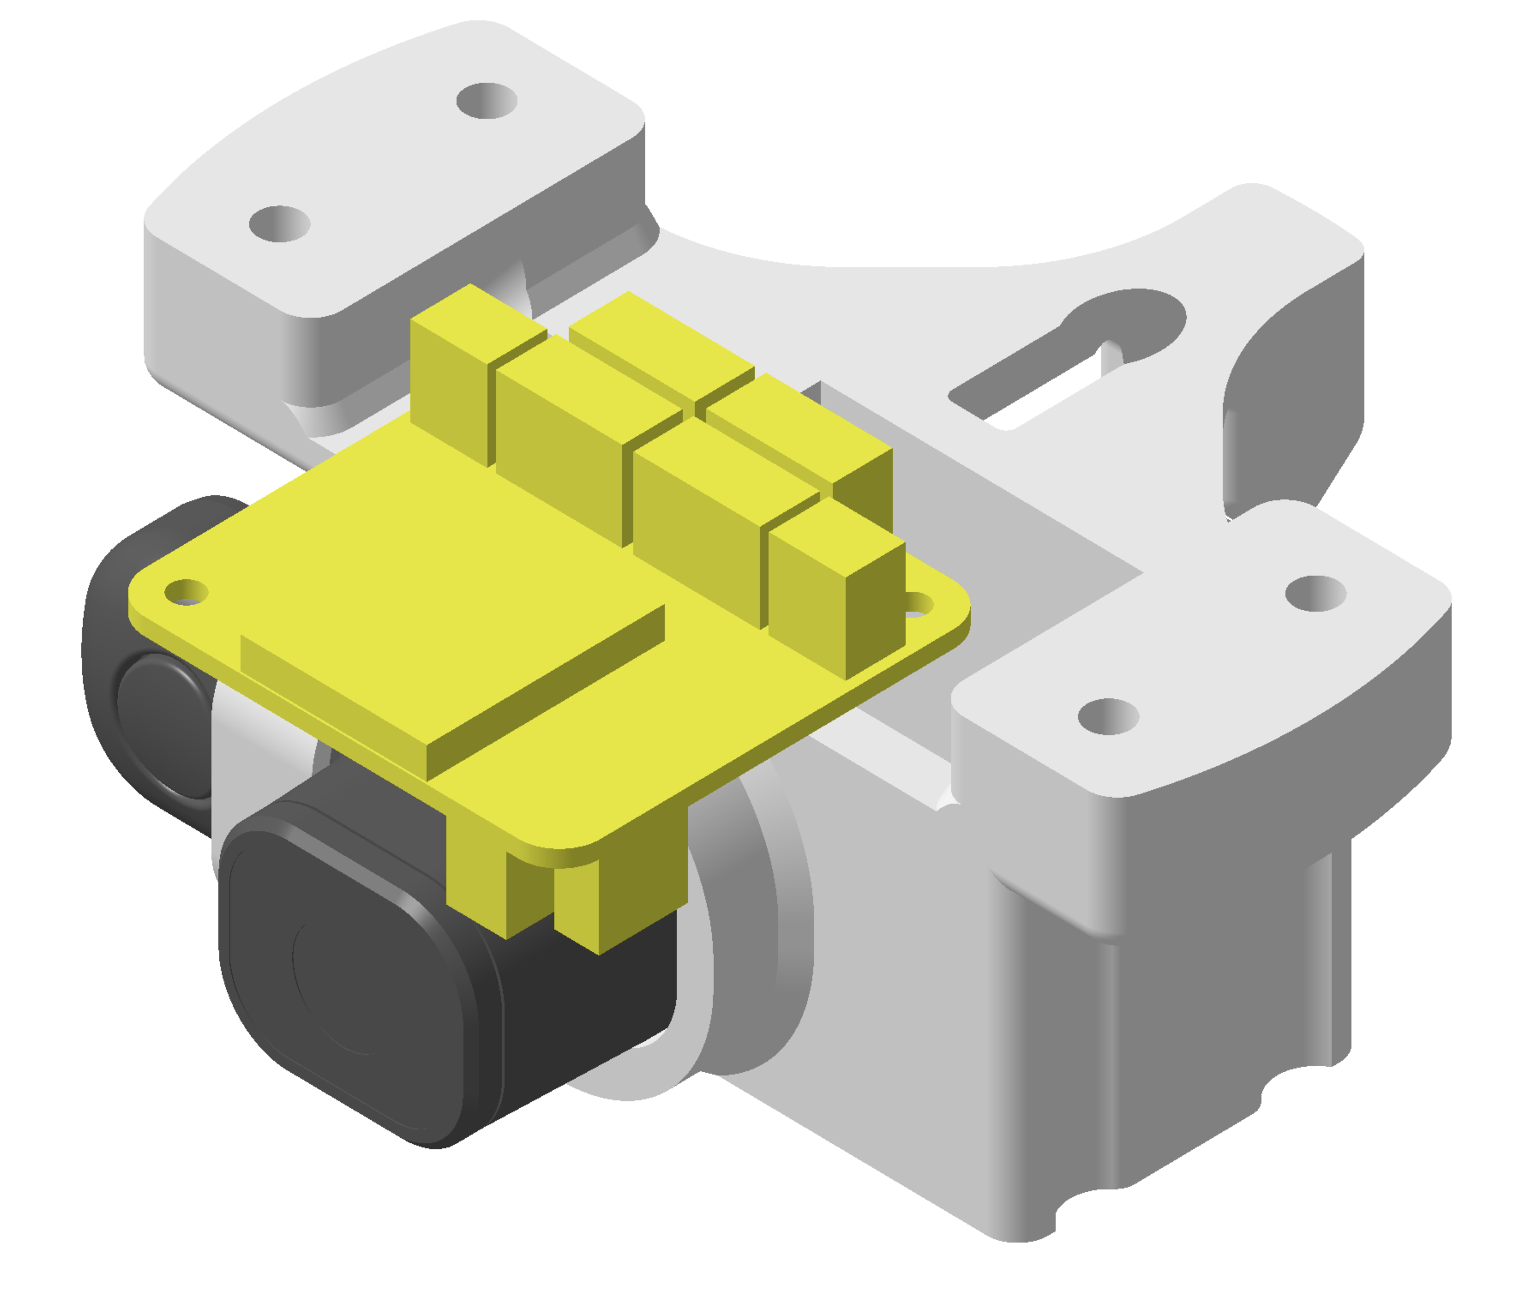
\includegraphics[width=0.45\linewidth]{figures/meca/support_runcam_ET1_1.png}\hfill
        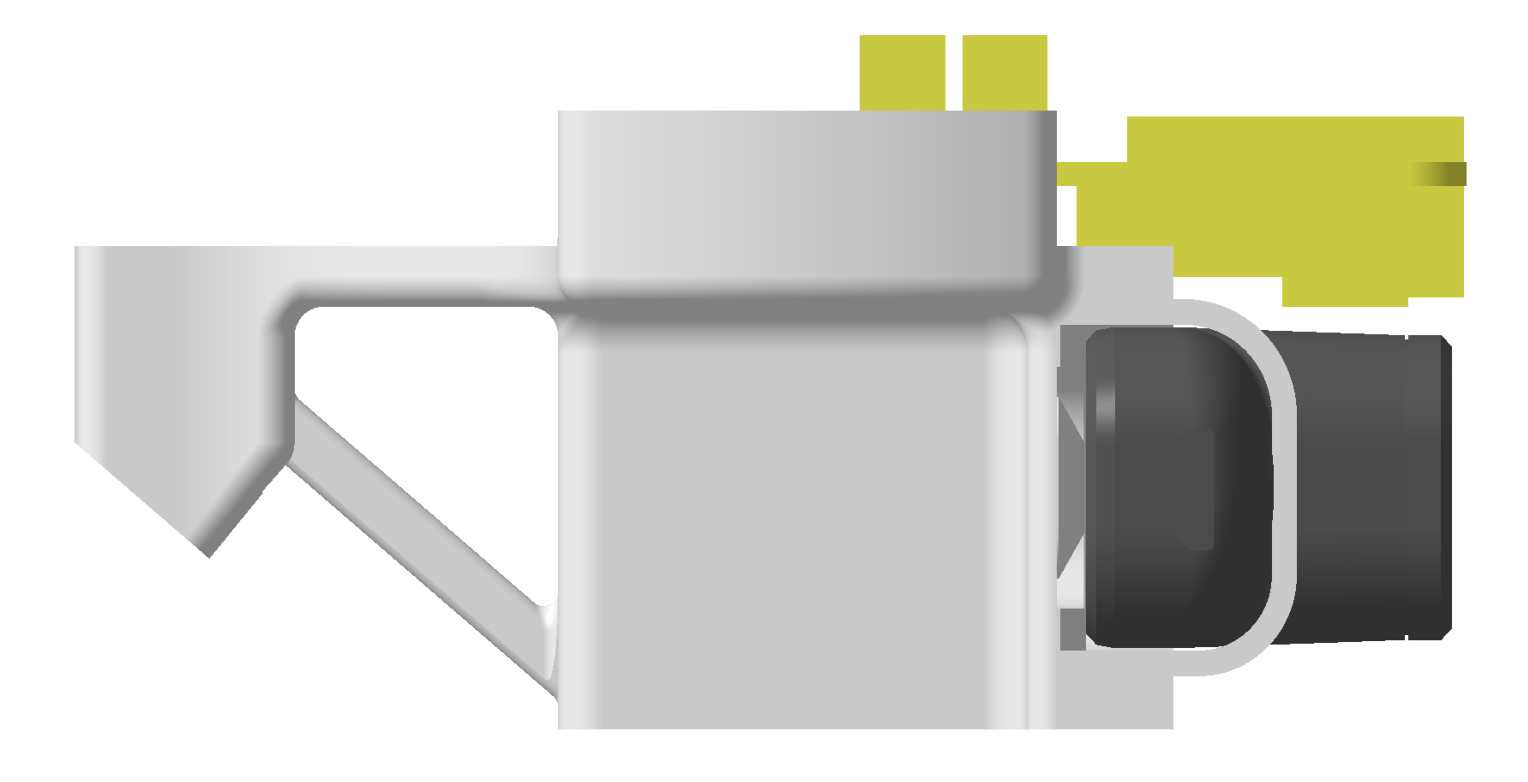
\includegraphics[width=0.45\linewidth]{figures/meca/support_runcam_ET1_2.png}\\[0.08cm]
        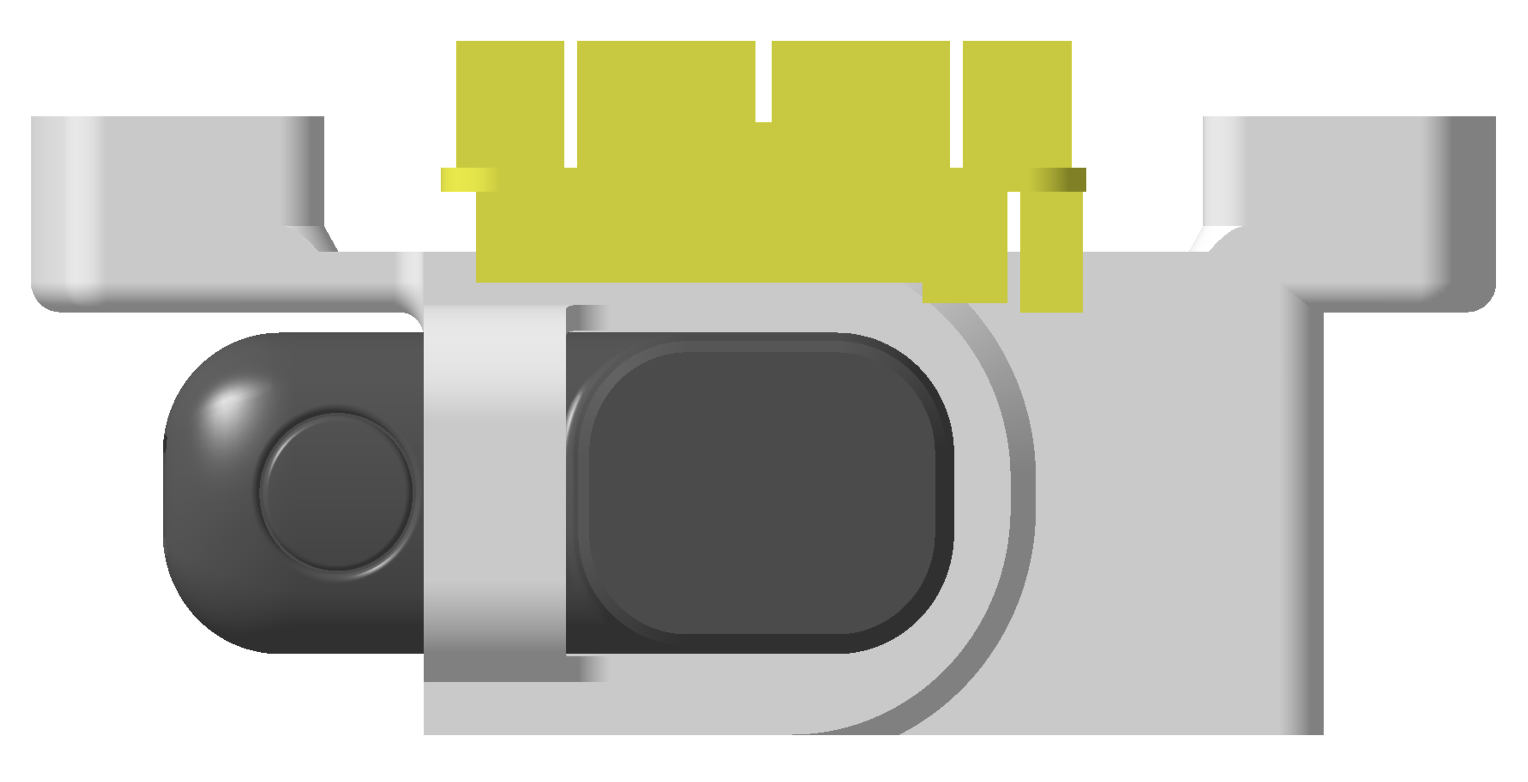
\includegraphics[width=0.45\linewidth]{figures/meca/support_runcam_ET1_3.png}\hfill
        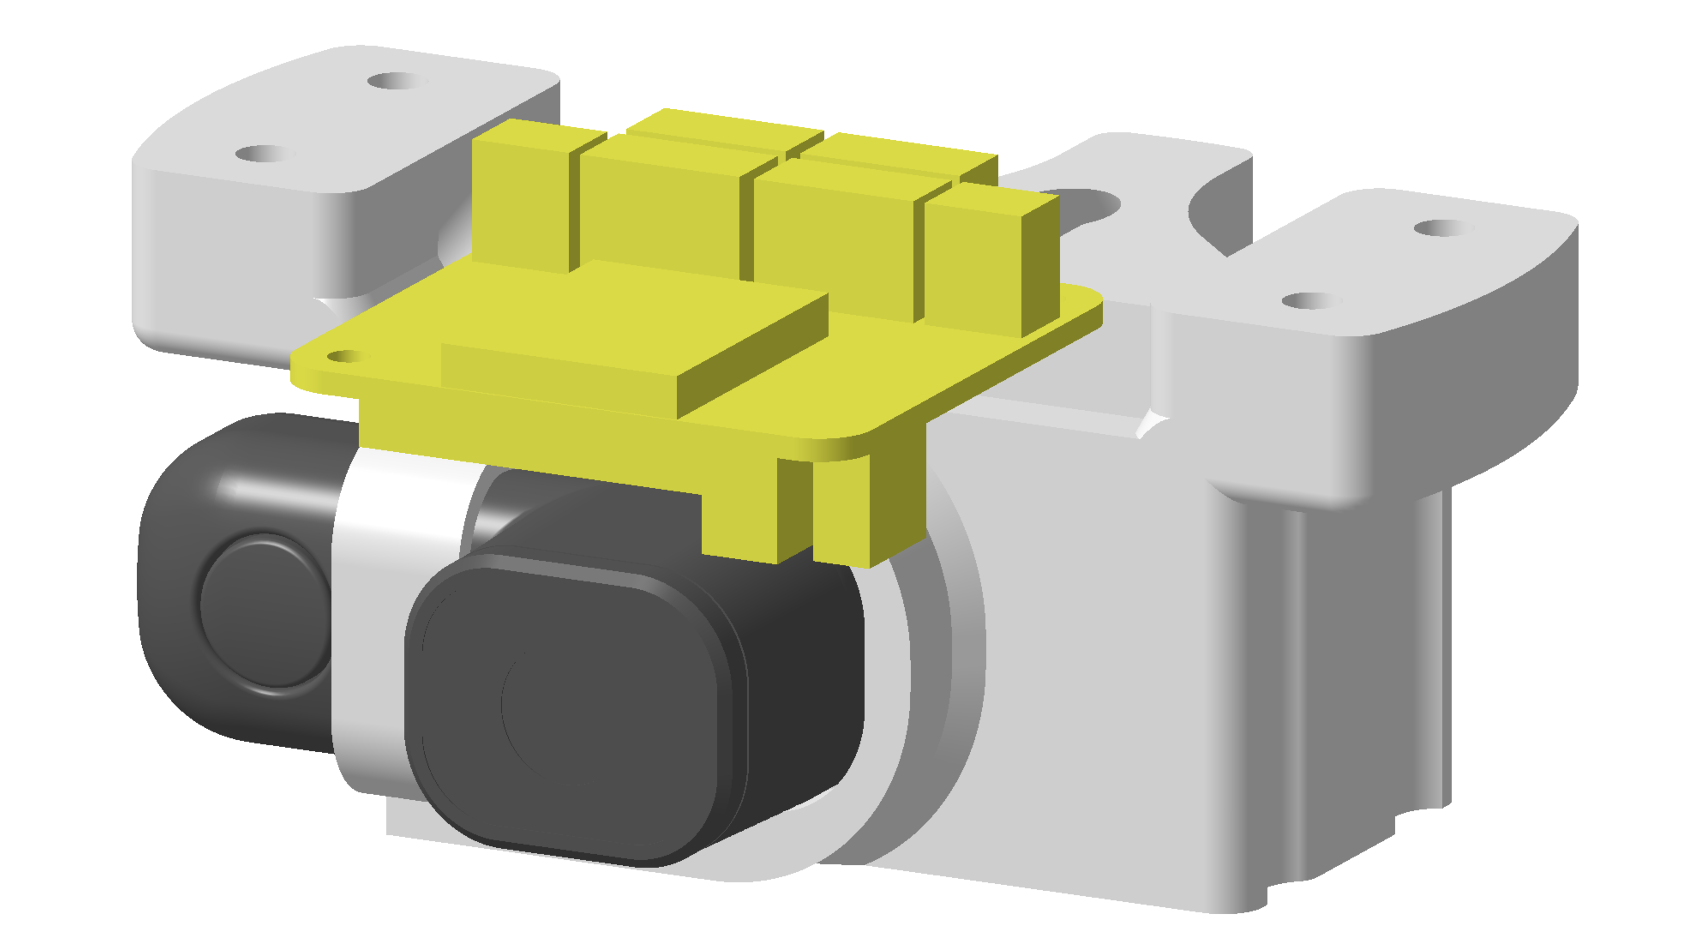
\includegraphics[width=0.45\linewidth]{figures/meca/support_runcam_ET1_4.png}
    \end{minipage}
    \caption{Mosaïque des quatre vues du support de la RunCam Thumb Pro du premier étage. La pièce jaune correspond à la PCB dédiée aux caméras.}
    \label{fig:support_thumb_etage1}
\end{figure}

\begin{figure}[H]
    \centering
    \begin{subfigure}[t]{0.48\textwidth}
        \centering
        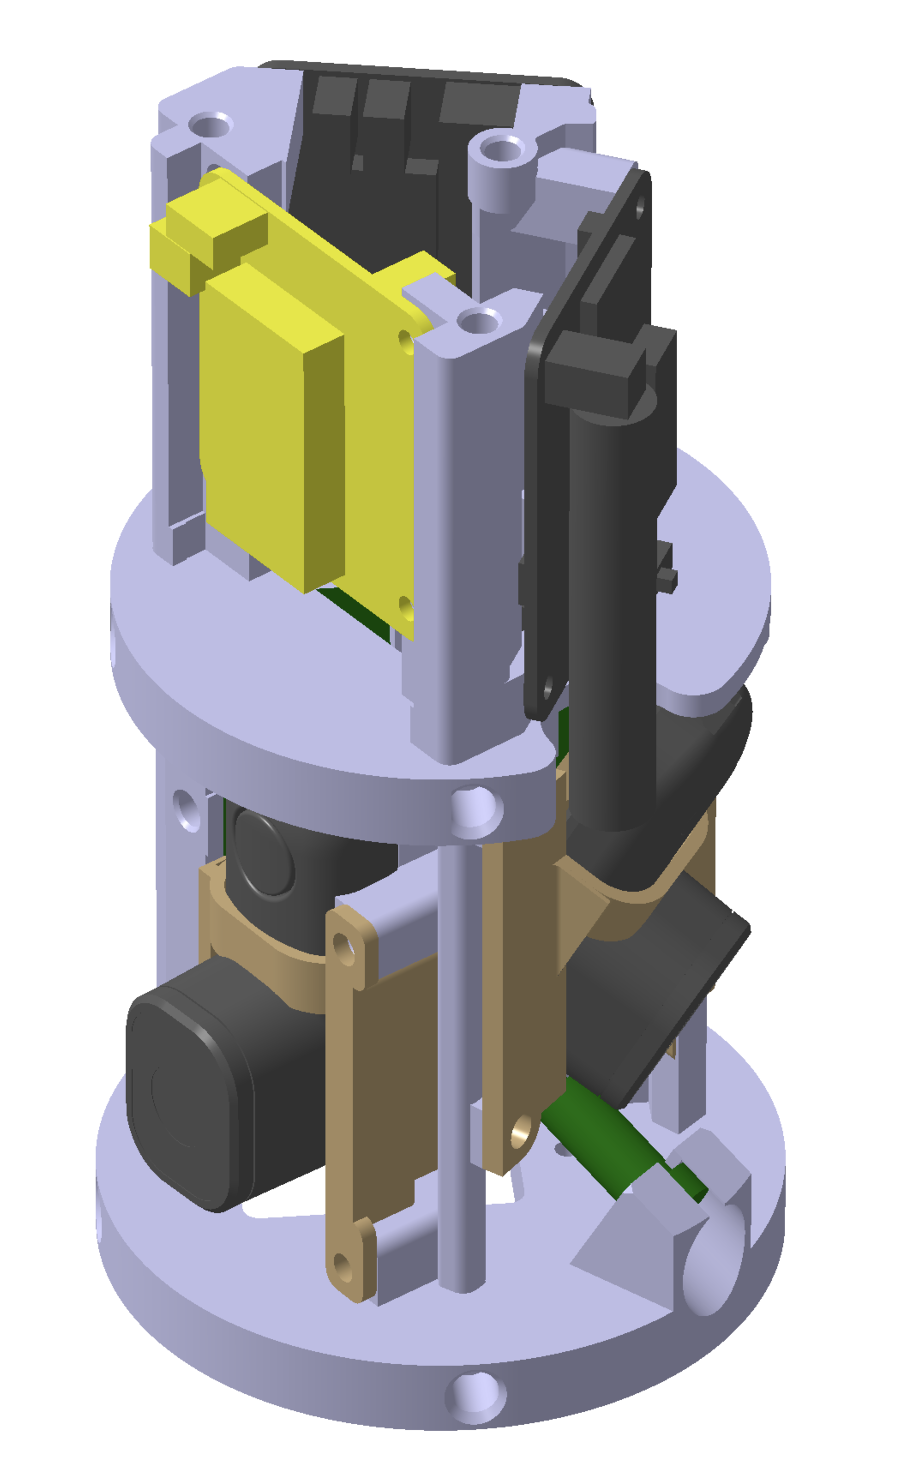
\includegraphics[width=0.75\linewidth]{figures/meca/support_runcam_ET2.png}
        \caption{Vue du bloc électronique.}
        \label{subfig:support_thumb_etage2_a}
    \end{subfigure}
    \hfill
    \begin{subfigure}[t]{0.48\textwidth}
        \centering
        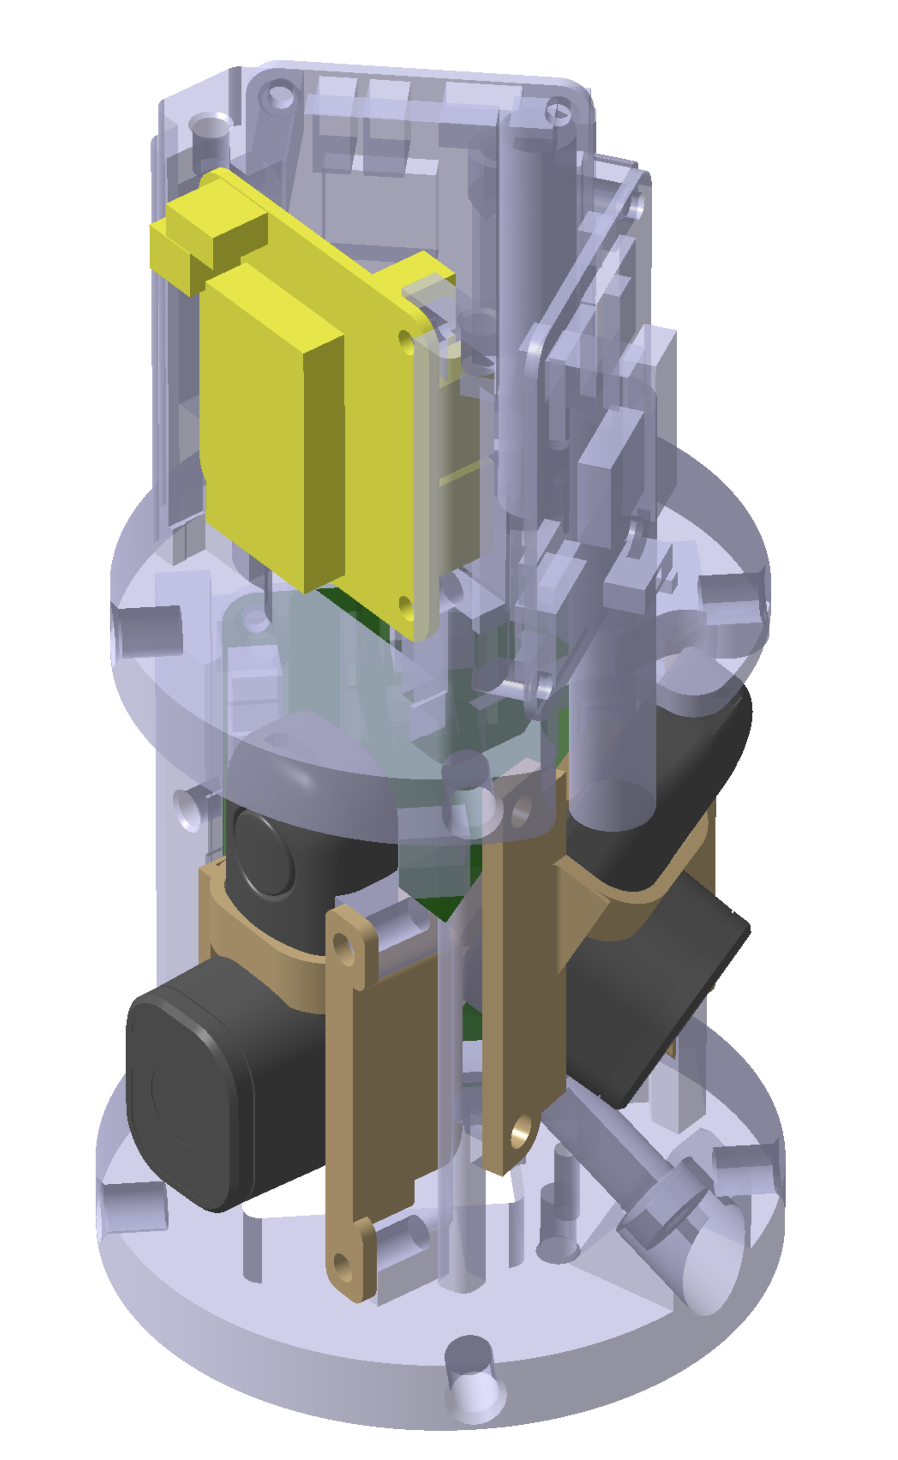
\includegraphics[width=0.75\linewidth]{figures/meca/support_runcam_ET2_transparent.png}
        \caption{Bloc rendu transparent.}
        \label{subfig:support_thumb_etage2_b}
    \end{subfigure}
    \caption{Vues du support des RunCam Thumb Pro du deuxième étage. Les supports apparaissent en marron et la PCB caméra en jaune.}
    \label{fig:support_thumb_etage2}
\end{figure}

\newpage

\subsubsection{RunCam Nano 2 dans la séparation inter-étages}

Les caméras sont fixées sur les différents blocs électroniques des baies avioniques. Des supports sur mesure ont été conçus
puis imprimés en 3D afin de maintenir chaque caméra et de garantir l'orientation voulue. Sur les vues d'intégration, les supports
de caméra apparaissent en marron et la PCB dédiée aux caméras en jaune. Cette représentation permet de visualiser la disposition
relative des caméras, de leur carte de commande et des blocs électroniques.\\

La comparaison des vues en coupe de la séparation met en évidence la différence d'encombrement entre l'Arducam OV2640,
prévue dans la conception initiale, et la RunCam Nano 2 finalement retenue. Cette dernière présente également un avantage
pour le positionnement de la caméra : son capteur est centré sur l'axe de la fusée et sur celui du moteur du deuxième étage.
La tuyère peut ainsi être maintenue dans le champ de vision sans décaler la caméra par rapport à l'axe longitudinal.\\

Cette caméra est destinée à observer la séparation des deux étages, ainsi que l'allumage et la mise en poussée du moteur du
deuxième étage. La vidéo permet également d'analyser a posteriori le comportement de la séparation et de comparer son
déroulement avec la modélisation mécanique.

\begin{figure}[H]
    \centering
    \begin{subfigure}[t]{0.48\textwidth}
        \centering
        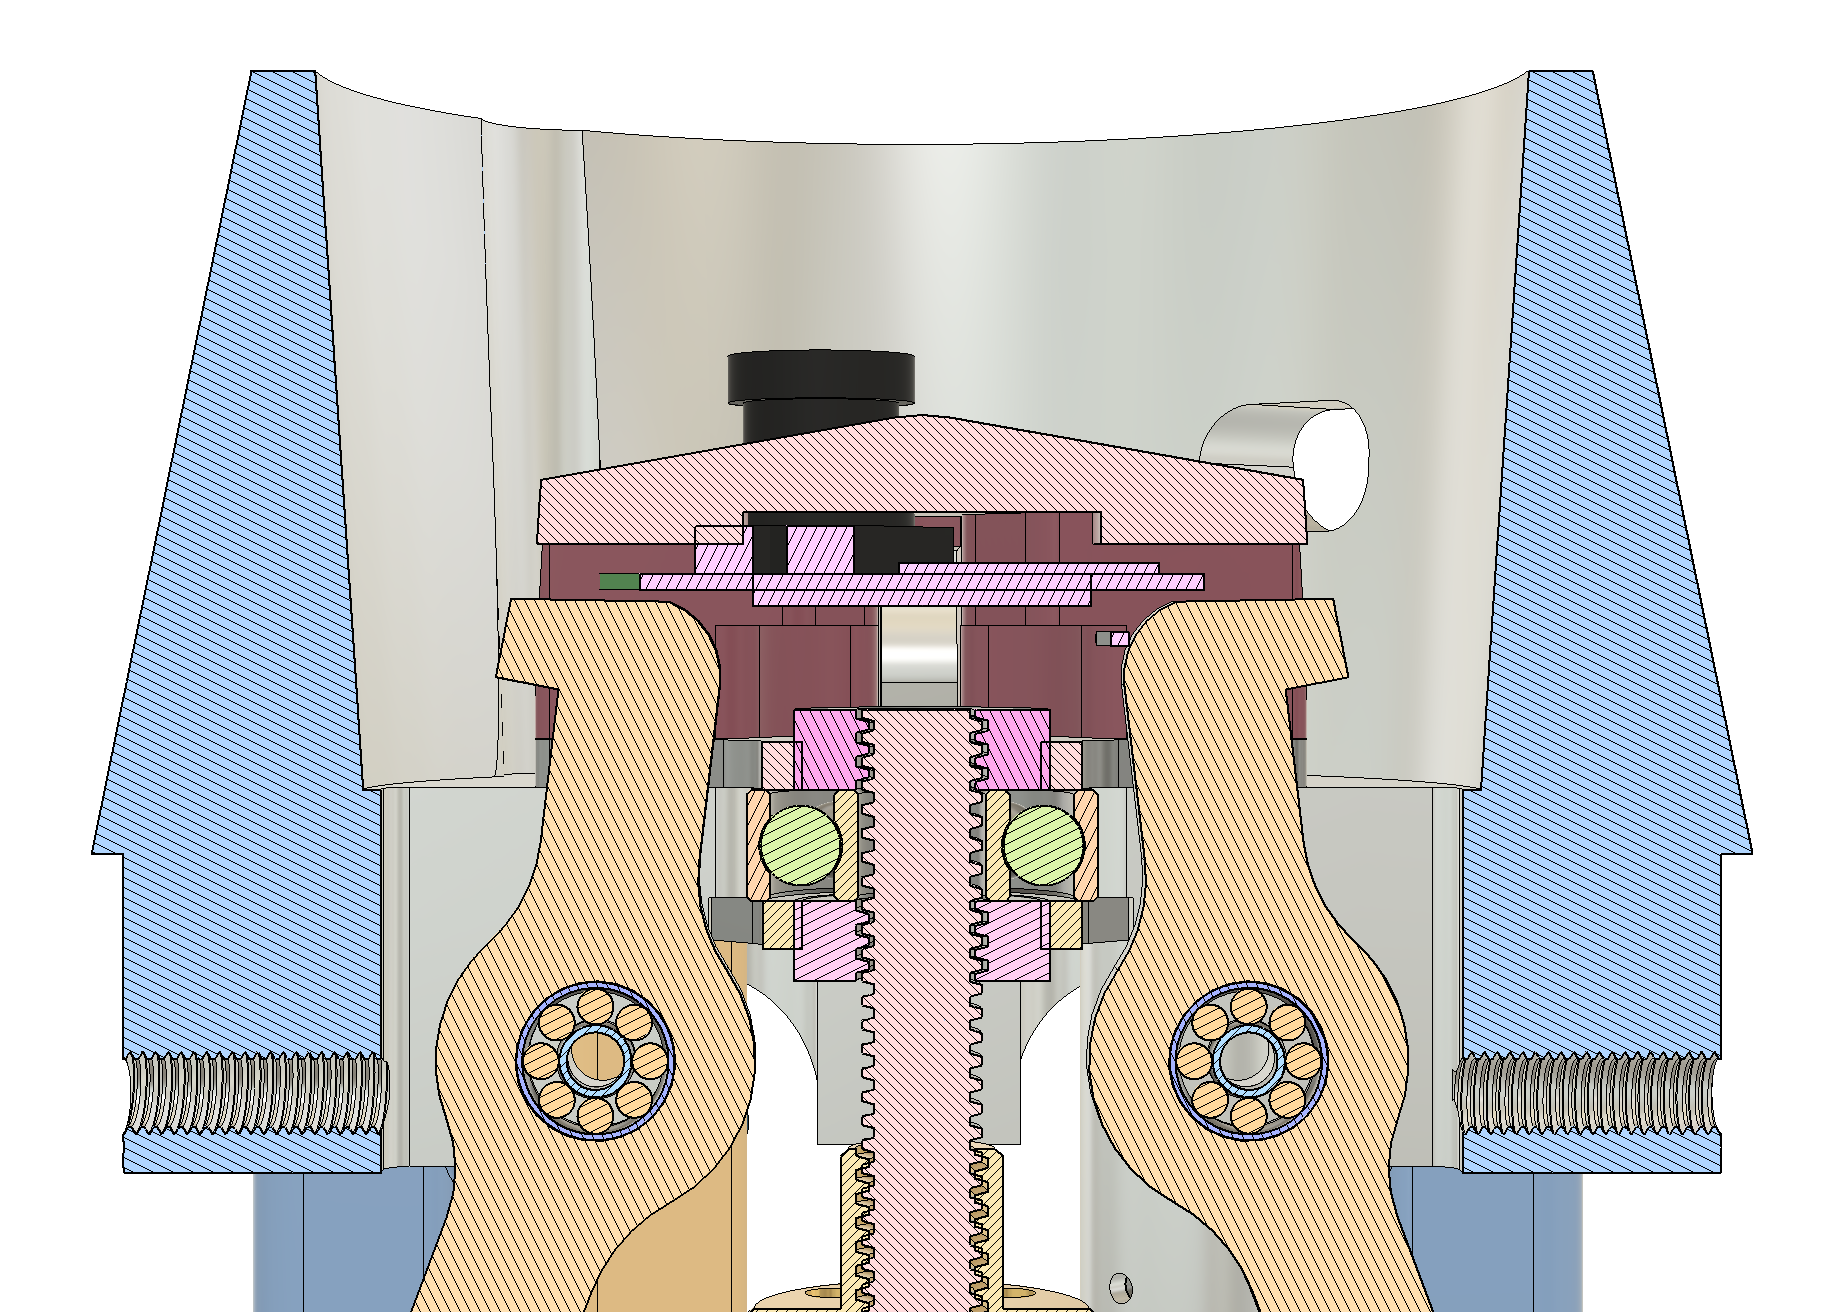
\includegraphics[width=\linewidth]{figures/meca/sepa_arducam.png}
        \caption{Arducam OV2640.}
        \label{subfig:coupe_separation_arducam}
    \end{subfigure}
    \hfill
    \begin{subfigure}[t]{0.48\textwidth}
        \centering
        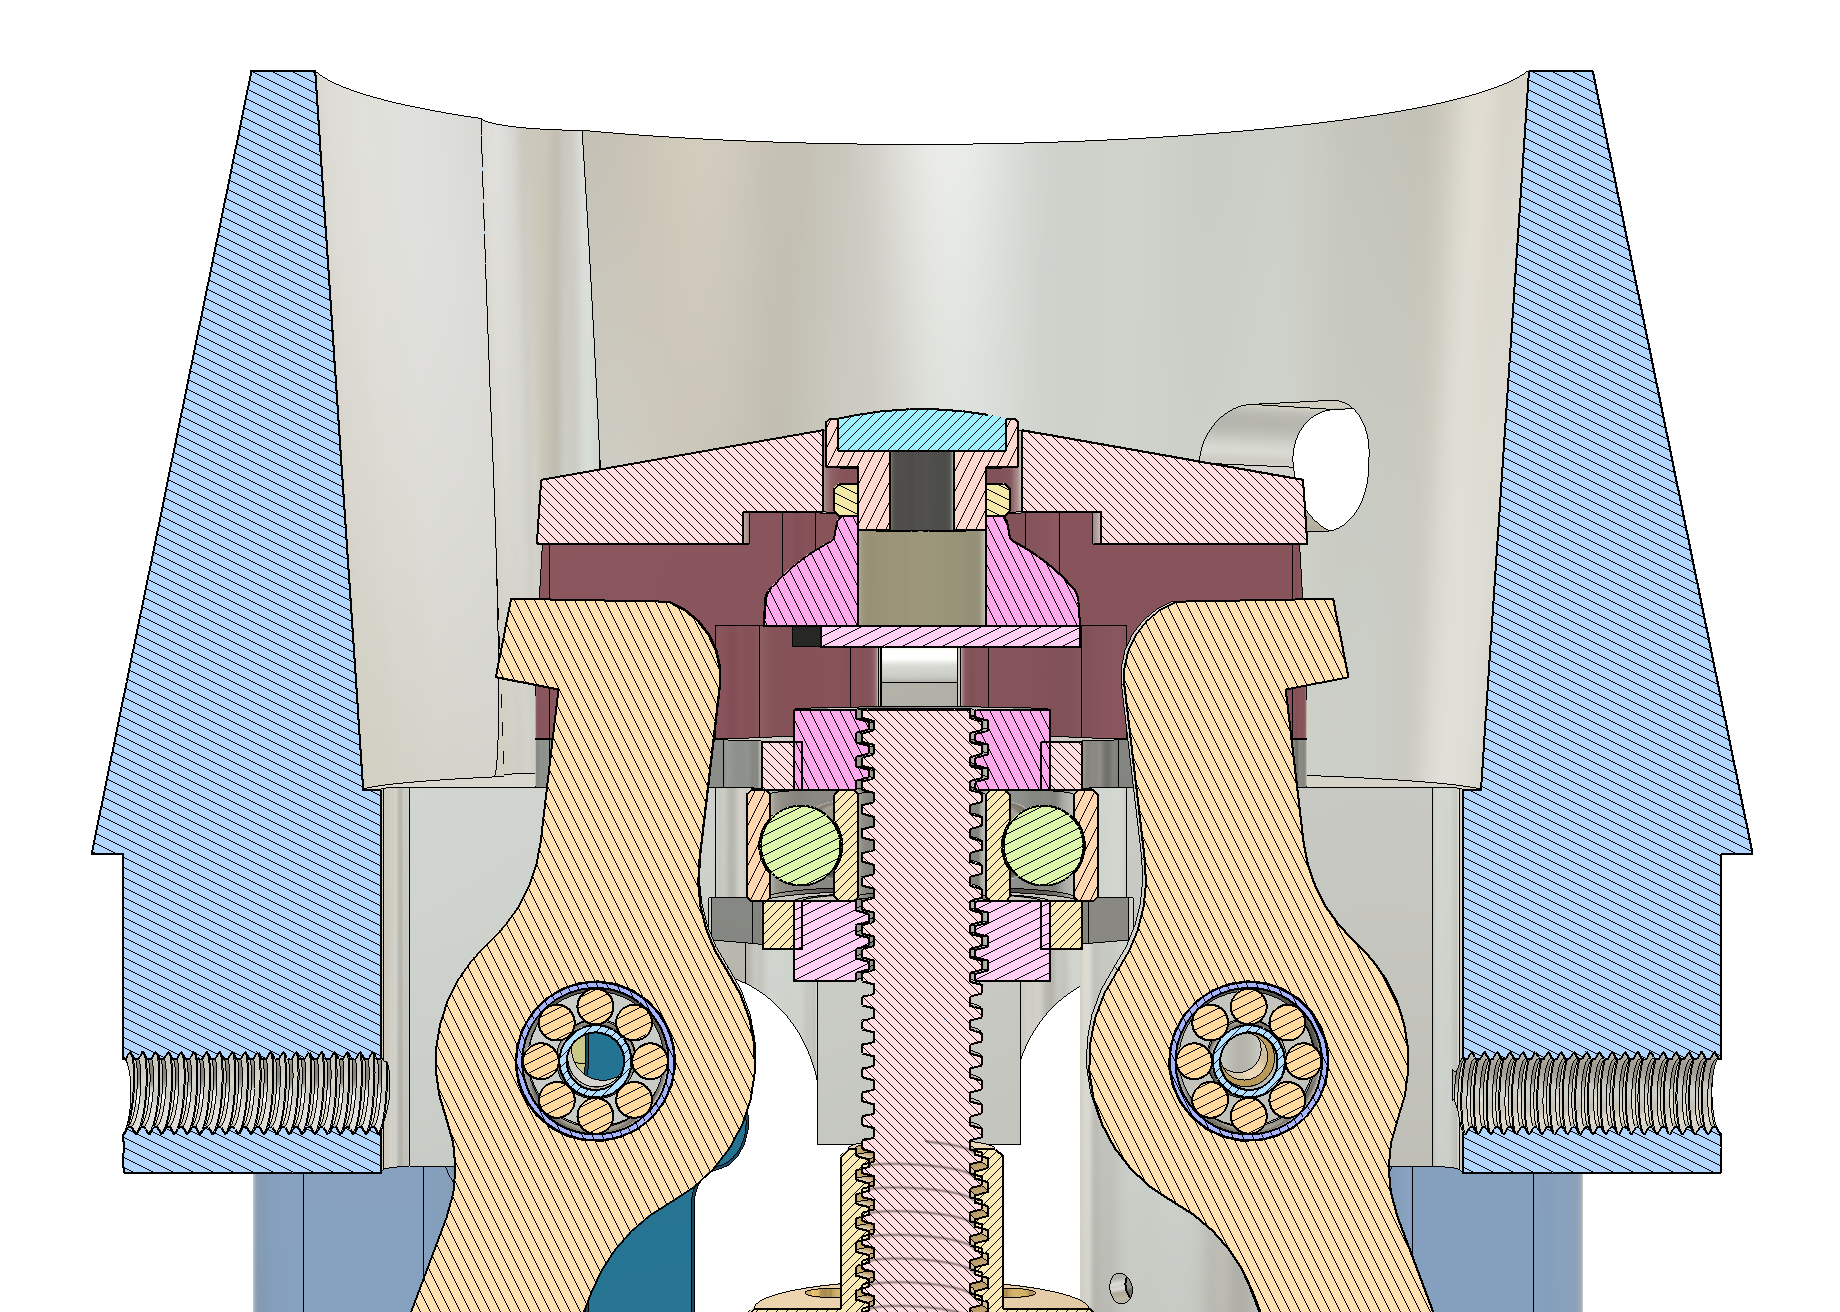
\includegraphics[width=\linewidth]{figures/meca/sepa_runcam_nano2.png}
        \caption{RunCam Nano 2.}
        \label{subfig:coupe_separation_nano2}
    \end{subfigure}
    \caption{Comparaison de l'encombrement des caméras dans la séparation inter-étages.}
    \label{fig:coupe_separation_camera}
\end{figure}

\begin{figure}[H]
    \centering
    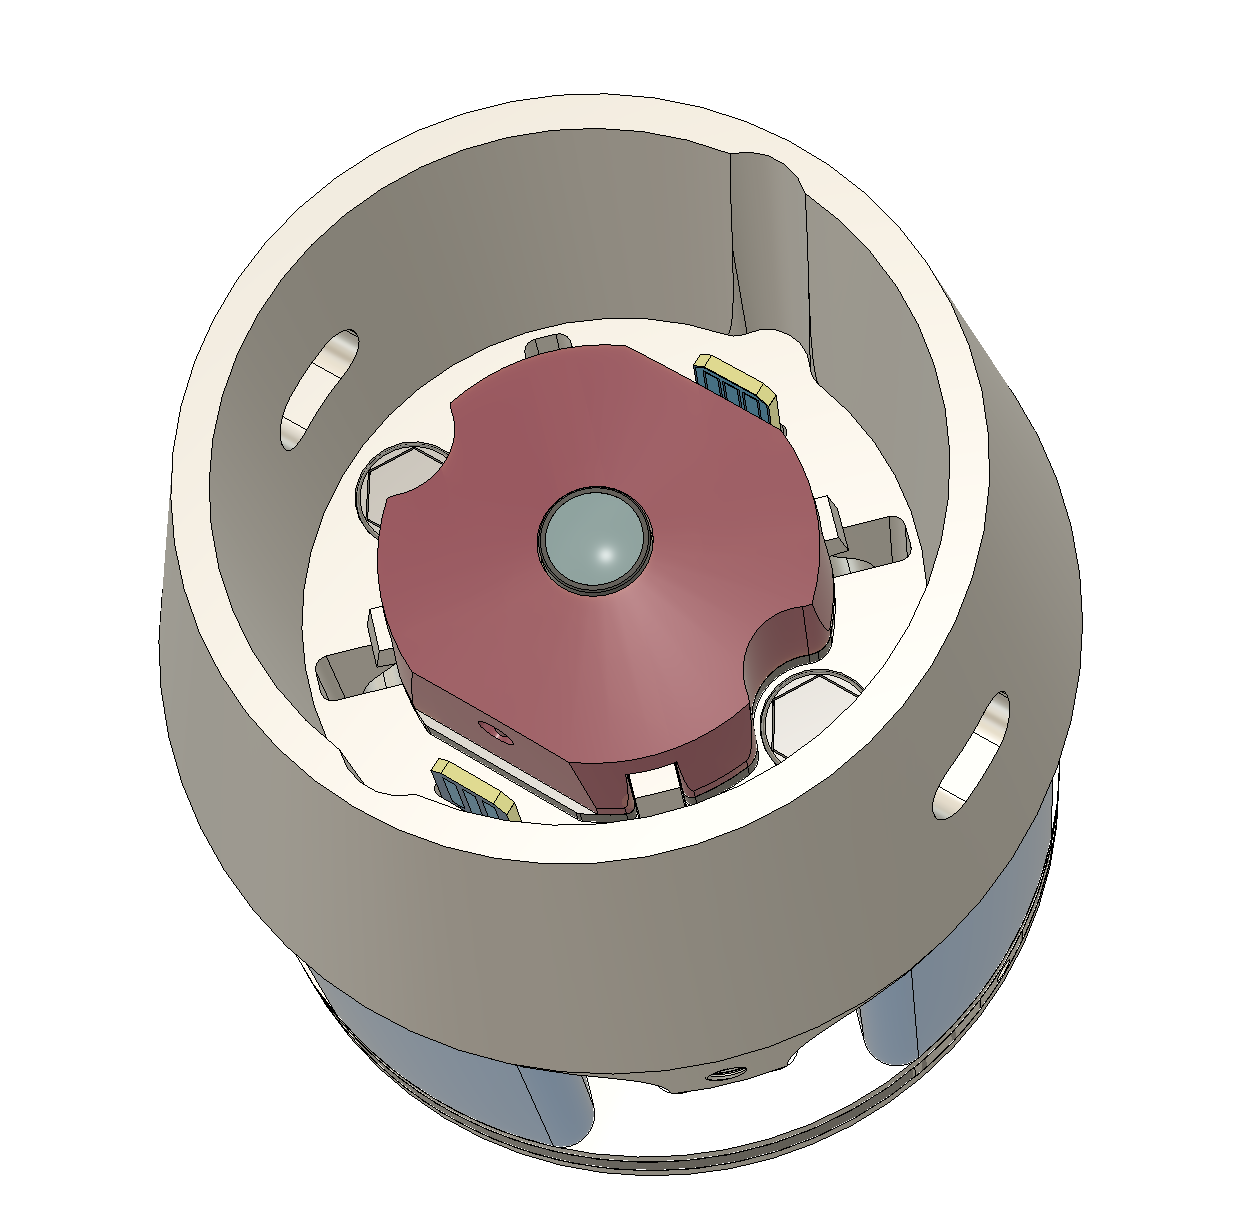
\includegraphics[width=0.55\textwidth]{figures/meca/support_sepa_nano2.png}
    \caption{Support de la RunCam Nano 2 intégré dans la séparation inter-étages.}
    \label{fig:support_nano2}
\end{figure}

\newpage
